%!TEX root = ../main.tex
\raggedbottom
\chapter{Background Study}
\label{chap:background_study}
This chapter presents a review of the research done on different aspects of phishing. It starts by defining the research methodology used and continues with a further articulation of the issue at hand. In doing so, it views phishing from the attacker's standpoint and profiles the victim. For the remainder of it, the chapter presents the most relevant research done in the area and offers critical appraisal on the work it outlines.


\section{Research methodology}
\label{sec:research_methodology}
The subject and aim of the research and literature review shifted several times throughout carrying out the required work. However, the aim has continuously been to develop an in-depth and high-resolution image of the subject matter and base the work presented in literature rather than suppositions. Throughout this dissertation, the systematic process used in doing the literature review is comprised of two procedures.

The first procedure dictates that the research should begin by firstly identifying a reputable and well-established study based on the number of references. This paper is thoroughly read, and the information relevant is extracted and processed accordingly.
The second procedure is used to deepen the understating of the subject. Based on the paper identified by procedure one, the points of interest are followed by spidering through references. When the process of spidering brings in focus papers less relevant to the aim, the research should return to procedure one.

Following this method ensures that by the end of the research phase, there will be a clear and in-depth understanding of the status quo in the subject of interest. Besides, the papers included in this chapter have received a greater level of attention to produce a pertinent appraisal of the work they present.


\section{Understanding the popularity}
\subsection{Attacker's viewpoint}
\label{subsec:attackers_viewpoint}
In understanding why phishing attacks are so popular amongst attackers, it is useful to view it from their perspective. A successful phishing attack circumvents most of a user's or enterprise's lines of defence. Most security solutions are centred around detecting and preventing actions that have not been explicitly initiated or allowed by the user. The critical issue is that a phishing attack, by definition, tricks the user into giving such information or carrying out the actions intended by the threat actor.

Other appealing factors for the attacker are the inherent vulnerabilities and proclivities of people. \cite{Ana_Ferreira} have brought together previous research on the subject to produce a list of principles of persuasion used in phishing attacks. By looking at the first contact with the possible victim, namely the email subject line, the study outlines that the most popular means of persuasion employed by attackers are: Authority (32.24\%), Strong affect (15.01\%) and Reciprocation (12.42\%). Given the amount of time phishing attacks have had to evolve organically, we can be confident in saying that these instruments gained popularity based on their positive influence on attack success.

\begin{figure}[!b]
	\centering
	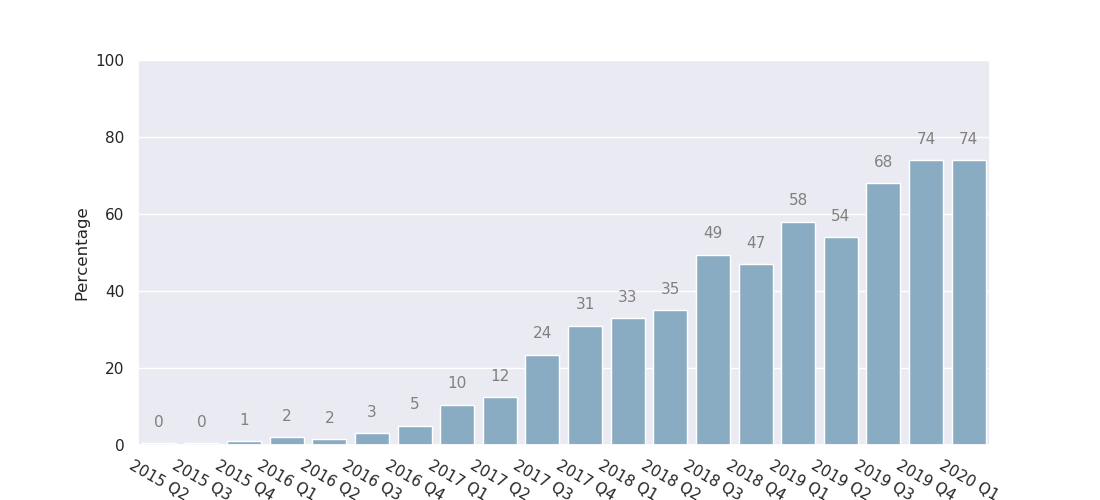
\includegraphics[width=1\textwidth]{apwg_https_usage.png}
	\caption{
		Reported number of phishing pages served over HTTPS \citep{APWG_Q42019}}
	\label{fig:HTTPS_USAGE}
\end{figure}


\subsection{Identifying the victim}
\label{subsec:identifying_the_victim}
To further the understanding of why phishing attacks are prevalent, we need to outline the profile of the victim. A well-established study of the victim is done by \cite{Rachna_Dhamija} which concludes the research by stating that there is no correlation between sex, age, education, browser, operating system, website used or hours of computer usage and the predisposition of being the victim of a phishing email. One unexpected discovery is that even in the best-case scenarios when the subject is expecting a phishing attack, the best phishing website deceived 90\% of the participants. The same research also describes the elements that users look after before trusting the website, the key takeaways being that 59\% of the participants based their decision on the page content, with some of them (36\%) paying little attention to the address bar. The rest of 41\% based their decision on the page content and domain name, but also the presence of HTTPS, the padlock icon and Secure Socket Layer (SSL) certificates.

\begin{table}[b]
	\begin{center}
		\begin{tabular}{  m{12em}  m{12em}  m{11.5em}  } \toprule
			                                  & \textbf{Highly susceptible} & \textbf{Less susceptible} \\ \midrule

			\textbf{Age}                      & 18-24 years old or less     & 25 years old or more      \\

			\textbf{Gender}                   & Female                      & Male                      \\

			\textbf{Anti-phishing training}   & No training                 & Anti-phishing trained     \\

			\textbf{Education}                & Humanities                  & Computer science          \\


			\textbf{Training delivery method} & Non-embedded                & Embedded                  \\

			\textbf{Personality}              & Agreeableness               & Consciousness             \\

			\textbf{Internet usage behaviour} & E-commerce and banking      & E-mails and browsing      \\ \bottomrule
		\end{tabular}

		\caption{\cite{Darwish} on susceptibility of being a victim of phishing}
		\label{tab:SUSCEPTIBILITY_BREAKDOWN}
	\end{center}
\end{table}

Since this research has been done, awareness of what HTTPS is and its importance have grown substantially, but so did the number of phishing websites using it. The launch date of the Electronic Frontier Foundation's \citep{EFF} certificate authority which provides SSL certificates at no cost can be correlated to \cite{APWG_Q42019}'s reported growing HTTPS adoption in serving phishing websites (Figure \ref{fig:HTTPS_USAGE}). This is especially dangerous and confusing for the victim as HTTPS is defined as secure Hypertext Transport Protocol (HTTP) and provides the icon of a green padlock, creating the feeling of a safe and secure website.

Other studies ventured to find correlations between personality particularities and the susceptibility of being deceived by a phishing attack, but they often are in direct contradiction. \cite{Darwish} managed to link the susceptibility of being deceived by a phishing attack to a set of arbitrary characteristics. The research concluded with the description of the two extremes of the spectrum, as shown in Table \ref{tab:SUSCEPTIBILITY_BREAKDOWN}.

In another study, \cite{Tzipora_Halevi} concluded that conscientiousness is the biggest indicator of the predisposition of being deceived by a phishing attempt. This is in direct opposition to the conclusion of \cite{Darwish}, which identifies agreeableness as the most accurate indicator of high susceptibility. Furthermore, it shows conscientiousness as the best indicator for low susceptibility of being a victim.


\section{Literature Review}
\label{sec:literature_review}
There is a wealth of approaches in phishing detection and prevention presented by the literature. To better visualize them, \cite{Sahingoz_Ozgur} synthesised the anti-phishing detection systems' literature structure, as shown in Figure \ref{fig:SOLUTION_CATEGORIES}. The following subsections focus the discussion on software-based, as user awareness is considered out of scope for this dissertation.

The literature review is categorised in rule-based (including blacklists, whitelists and heuristics) and machine learning-based. Some solutions do have some hybrid aspects but have been assigned to the category considered as most relevant. The reason behind the selected categories lies in the fundamentally different type of classification mechanism.

\begin{figure}[t]
	\centering
	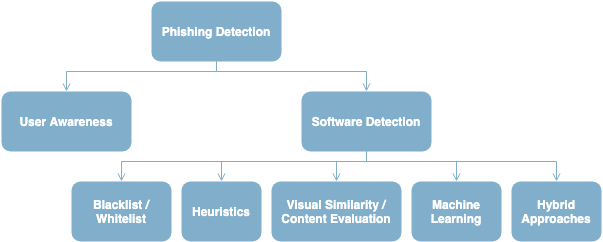
\includegraphics[width=0.9\textwidth]{phish_detection_class.png}
	\caption{
		Categorisation of prevention solutions
		\citep{Sahingoz_Ozgur}}
	\label{fig:SOLUTION_CATEGORIES}
\end{figure}

\subsection{Rule-based phishing detection}
\label{subsec:rule-based_detection}
Rule-based phishing solutions classify websites as malicious or legitimate based on a pre-defined set of rules. Because the ruleset is the centrepiece of the detection system, the resulted performance is tightly linked to its design. As a consequence, the focus is set on rule selection and conditional relationship setting.

\cite{Ye_Cao} proposed an automated individual whitelist capable of updating itself with records of the IP addresses of each website visited which features a login page. If the user attempts to submit information through such a login user interface, they get a warning informing them that they are doing so on a webpage outside of the whitelist. The proposed solution uses the Naive Bayesian classifier to take decisions, which has delivered high effectiveness in previous studies on anti-spam \citep{Ion_Androutsopoulos} and junk email \citep{Mehran_Sahami} filters. After the decision has been taken, the classification is expected to be further confirmed by the user. Although the proposed solution delivered a rate of true positives of 100\% and a rate of false negatives of 0\%, the disadvantage is that this approach relies on the involvement of the user, and cannot discover new phishing webpages.

Another whitelist based approach is presented by \cite{Jain}, which achieves phishing detection using a two-phase method. The proposed system logically splits webpages into "not visited" and "re-visited". The first module is triggered when a page is re-visited and consists of a domain lookup within the whitelist. If the domain name is found, the system matches the IP address to deliver the decision. When the domain name cannot be found in the whitelist, the system uses a statistical analysis of the number of hyperlinks pointing to a foreign domain. After extraction, the system examines the features from the hyperlinks to take the decision. Although the proposed system covers a variety of phishing attacks (e.g. DNS poisoning, embedded objects, zero-hour attack), it has declared experimental results of 86.02\% true-positive rate and 1.48\% false-negative rate.

\cite{Yue_Zhang} proposed an adaptation of the term frequency-inverse document frequency (TF-IDF) information retrieval algorithm for detecting phishing webpages in a content-based approach called CANTINA. The solution uses the TF-IDF algorithm to extract the most frequently used five words, which are then fed into a search engine. The website's domain name is then compared with the top \(N\) domain names resulted from the search, and if there is a match, the website is labelled as legitimate.
To lower the rate of false-positives, they included a set of heuristics checking the age of the domain, the presence of characters such as '@' signs, dashes, dots or IP addresses in the URL. Furthermore, it features some content-based checks such as inconsistent well-known logos, links referenced and forms present. The experimental results show a true positive rate of 97\% and a false positive rate of 6\%. After the addition of these heuristics, the false positive rate decreased to 1\% but so did the true positive rate, which decreased to 89\%. An important note about this research is that the resulted effectiveness is tightly linked to the English language.

\cite{Rami_Mohammad} presents an intelligent rule-based phishing detection system, whose ruleset is produced through data mining. The study begins with a proposed list of seventeen phishing features derived from previous work on anti-phishing detection systems. These are then fed into different rule-based classification algorithms, each of which utilises a different methodology in producing knowledge. The conclusion presents C4.5 \citep{Quinlan} as the algorithm that produced the most effective ruleset. The extracted set presents features related to the request URL, age of the domain, HTTPS and SSL, website traffic, subdomain and multi subdomain, presence of prefix or suffix separated by "--" in the domain and usage of IP addresses. The downside of this solution is the reliance on third-party services providing information about the age of the domain, webpage traffic, and DNS record data. Furthermore calibrating the thresholds for each feature requires complex statistical work.

\begin{singlespace}
	\begin{table}[!b]
		\small
		\begin{center}
			\begin{tabular}{ m{41.5em} }\toprule
				\\
				\(Rule\ 1: if\ \{\ Transport\ Layer\ Security\ =\ HTTP\ \cap\ Keyword\ in\ the\ path\)

				\(portion\ of\ the\ URL\ =\ yes\ \cap\ Top\ Level\ Domain\ =\ yes\ \}\ \implies\ class\ phishing\)
				\\\\
				\(Rule\ 2: if\ \{\ Number\ of\ slashes\ in\ URL\ \geq\ 5\ \cap\ Transport\ Layer\ Security\ =\ HTTP\ \cap\ Keyword\ in\ the\ path\ of\ the\ URL\ =\ yes \}\ \implies class\ phishing\)
				\\\\
				\(Rule\ 3: if\ \{\ Special\ characters\ =\ yes\ \cap\ Transport\ Layer\ Security\ =\ HTTP\ \cap\ Number\ of\ terms\ in\ the\ host\ name\ of\ the\ URL\ > 4\ \}\ \implies class\ phishing\)
				\\\\
				\(Rule\ 4: if\ \{\ Dots\ in\ the\ host\ URL\ > 4\ \cap\ Transport\ Layer\ Security\ =\ HTTP\ \cap\ Number\ of\ terms\ in\ the\ host\ name\ of\ the\ URL\ > 4\ \}\ \implies class\ phishing\)
				\\\\
				\(Rule\ 5: if\ \{\ Number\ of\ slashes\ in\ URL\ \geq 5\ \cap\ Dots\ in\ the\ host\ URL\ > 4\ \cap\ Length\ of\ the\ URL\ > 75\ \}\ \implies class\ phishing\)
				\\\\
				\(Rule\ 6: if\ \{\ Special\ characters\ =\ yes\ \cap\ Transport\ Layer\ Security\ =\ HTTP\ \cap\ Top\ Level\ Domain\ =\ yes\ \}\ \implies class\ phishing\)
				\\\\
				\(Rule\ 7: if\ \{\ Dots\ in\ the\ host\ URL\ > 4\ \cap\ Transport\ Layer\ Security\ =\ HTTP\ \cap\ Keyword\ in\ the\ path\ of\ the\ URL\ =\ yes\ \}\ \implies class\ phishing\)
				\\\\
				\(Rule\ 8: if\ \{\ Special\ characters\ =\ yes\ \cap\ Transport\ Layer\ Security\ =\ HTTP\ \cap\ Keyword\ in\ the\ path\ of\ the\ URL\ =\ yes\ \}\ \implies class\ phishing\)
				\\\\
				\(Rule\ 9: if\ \{\ Dots\ in\ the\ host\ URL\ > 4\ \cap\ Keyword\ in\ the\ path\ of\ the\ URL\ =\ yes\ \cap\ Top\ Level\ Domain\ =\ yes\ \}\ \implies class\ phishing\)
				\\\\ \bottomrule
			\end{tabular}
			\caption{\label{tab:MINED_RULES}Rule mining results of the apriori algorithm \citep{Jeeva}}
		\end{center}
	\end{table}
\end{singlespace}

\cite{Jeeva} approaches phishing detection by firstly focusing on the extraction of quintessential indicators statistically proven to be found in phishing websites. The paper then presents a set of heuristics based on the aforementioned statistical investigations and analysis, which are translated into fourteen rules responsible for URL classification. Similar to \cite{Rami_Mohammad}, the identified rules are fed into two data mining algorithms (Apriori and Predictive Apriori), to discover meaningful associations between them. The paper concluded by stating the two sets resulted from associative rule mining, and the reported experimental accuracy of 93\% when using the ruleset mined by the apriori algorithm. The rules used to achieve this efficiency are presented in Table \ref{tab:MINED_RULES}.

\subsection{Machine-learning based phishing detection}
\label{subsec:machine-learning_based_phishing_detection}
Machine learning-based solutions centre around the processes of feature extraction and the training of machine learning models. These features take the shape of information from different parts of the website, such as the URL or the Hypertext Markup Language (HTML) content. This subsection will briefly discuss a variety of machine learning approaches to anti-phishing detection systems, and the essential takeaways from the
studies covered.

\cite{Le} proposes PhishDef --- a system which does on-the-fly classification of phishing URLs based on lexical features and adaptive
regularisation of weights (AROW) \citep{AROW}. The AROW algorithm offers the capability of calibrating the classification mechanism upon making a wrong prediction. As a result, the predictions will be of high accuracy even when the trained model is provided with noisy data. Furthermore, PhishDef uses an online classification algorithm, as opposed to a batch-based one. Online classification algorithms continuously retrain their model when encountering new data, instead
of just delivering the prediction. PhishDef reports an accuracy of 95\% with noise ranging from 5\% to 10\%, and above 90\% when noise is between 10\% to 30\%. A note worth mentioning is that PhishDef achieves the accuracy as mentioned earlier while having low computational and memory requirements.

Furthering the work on CANTINA mentioned in Subsection \ref{subsec:rule-based_detection}, \cite{Guang_Xiang} enhanced the detection system by adding a feature-rich machine learning module. The iteration is named CANTINA+, and it aims to address the high false-positive rate of its predecessor. Besides machine learning techniques, this enhanced iteration brings focus on search engines, and the HTML Document Object Model (DOM), adding several checks on brand, domain, hostname search and HTML attributes. Besides the inherited trade-offs of CANTINA, the research states that one of the limitations of CANTINA+ is the incapability of delivering predictions on phishing websites that are composed of images, thus offering no text for it to analyse. Furthermore, while it manages to improve upon the original implementation of CANTINA and successfully achieves an accuracy rate of 92\%, it is still prone to producing a considerable number of false positives.

\cite{Ling_Li} present a multi-stage detection system that aims to both pro-actively and reactively take action against banking bot-nets. The first feature of this model is an early warning detection module which supervises the malicious-looking newly registered domains. The second module does spear phishing detection using a machine learning model trained on different variations of popular domains such as bitsquatting, omission, and other alteration techniques. Although this research is focused more on banking bot-nets, the approach used in URL variations detection and spear-phishing protection is well designed. Furthermore, it shows how much such coverage over the lifecycle of a bot-net can achieve.

\cite{Li_Yukun} takes a different approach by utilising a stacked machine learning model that surpasses the capability of single model implementations of anti-phishing detection systems. The study shows the comparison between the proposed stack composed of Gradient Boosting Decision trees \citep{Jerome_Friedman}, XGBoost \citep{Tianqi_Chen}, and LightGBM \citep{Guolin_Ke} and single models using algorithms such as support vector machine, nearest neighbour classifier, decision trees, and random forest. Moreover, it provides a wealth of information about efficiency differences between different single or stacked models. To measure inter-rater reliability for qualitative (categorical) items and select the best candidates for the stacking model \cite{Li_Yukun} uses Cohen's kappa static \citep{Ian_Witten}. The resulted stack was selected based on the kappa as mentioned earlier, and the lower average error.
This method of selection lowered the false-positive and false-negative rates of the stacking model when compared to all its components individually. Finally, the research reports an accuracy rate of the stacked
model of 97.3\%. with a false positive of 1.61\% and a false negative rate of
4.46\%.

\cite{Sahingoz_Ozgur} investigates the possibility of a real-time anti-phishing system by training seven different classification algorithms with natural language processing (NLP), word vector and hybrid features. In doing so, \cite{Sahingoz_Ozgur} states the lack of a worldwide acceptable test dataset for effectiveness comparison between phishing solutions and proceeds to construct one containing 73,575 URLs of which 34,600 legitimate and 37,175 malicious. The paper uses this dataset to conduct comparisons between previous work in the field and the selected classification algorithms (Decision Trees, Adaboost, Kstar, K-Nearest Neighbour, Random Forest, Sequential Minimal Optimization and Naive Bayes), outlining the best performers. The most effective combination discovered is the Random Forst algorithm trained with NLP features. It achieved an experimental accuracy of 97.98\% in URL classification, while being language and third-party service independent, and achieving real-time execution and detection of new websites. A noticeable tendency emergent from the comparisons is that the NLP features seem to improve accuracy across the majority of machine learning algorithms covered.

\cite{Adebowale} studies the performance of a few machine learning models, one of which is an artificial neural network named Adaptive Neuro-Fuzzy Inference System \citep{Jang} when trained with integrated text, image, and frame features. The research presents a brief comparison between the proposed solution and numerous other anti-phishing detection systems which can be found in Table \ref{tab:EXISTENT_SOLUTIONS}.
Throughout its content, the paper builds a set of 35 features from phishing websites analysis and related work while also comparing their efficiency. These are then bound in sets and fed into ANFIS, SVM, and KNN algorithms to study the outcome.
The ANFIS-based hybrid solution (including text, image and frame features) delivered an accuracy of 98.30\%. Although the research considers the previously mentioned solution as the conclusive, the ANFIS text-based classification records an accuracy of 98.55\%. Besides this, throughout the

\begin{center}
	\small
	\begin{tabular}{  m{0.5em}  m{6em}  m{13.3em}  m{8.5em}  m{2.3em}  m{4.3em}  } \toprule

		                                & \textbf{Plugin } & \textbf{Features \& Techniques} & \textbf{Browser}    & \textbf{Acc} & \textbf{Type} \\ \midrule

		\multicolumn{1}{r}{\textbf{1}}  & GoldPhish        & Heuristics \& Features-based    & IE                  & 98           & Free          \\

		\multicolumn{1}{r}{\textbf{2}}  & Cloudmark        & Heuristics                      & IE                  & 94           & Free          \\

		\multicolumn{1}{r}{\textbf{3}}  & SmartScreen      & Blacklist and whitelist         & IE                  & 95.9         & Free          \\

		\multicolumn{1}{r}{\textbf{4}}  & Netcraft         & Blacklist and whitelist         & Chrome, Firefox     & 90           & Free          \\

		\multicolumn{1}{r}{\textbf{5}}  & SpoofGuard       & Heuristics \& Features-based    & IE                  & 91           & Free          \\

		\multicolumn{1}{r}{\textbf{6}}  & Phishdentity     & Google search-by-image API      & IE                  & 97.2         & Research      \\

		\multicolumn{1}{r}{\textbf{7}}  & PhishTackle      & Heuristics \& Features-based    & IE                  & 91.3         & Research      \\

		\multicolumn{1}{r}{\textbf{8}}  & PhishGuard       & Heuristics                      & Firefox             & 94           & Research      \\

		\multicolumn{1}{r}{\textbf{9}}  & PhishIdentifier  & Heuristics                      & Firefox             & 92           & Research      \\

		\multicolumn{1}{r}{\textbf{10}} & PhishTester      & Heuristics \& Features-based    & IE                  & 97.1         & Research      \\

		\multicolumn{1}{r}{\textbf{11}} & CANTINA+         & Heuristics \& Features-based    & IE                  & 98.06        & Research      \\

		\multicolumn{1}{r}{\textbf{12}} & PhishAri         & Features-based                  & Chrome              & 92.52        & Research      \\

		\multicolumn{1}{r}{\textbf{13}} & PhishShield      & Heuristics \& Feature-based     & Chrome              & 96.57        & Research      \\

		\multicolumn{1}{r}{\textbf{14}} & PhishNet         & Blacklist                       & Chrome              & 95           & Research      \\

		\multicolumn{1}{r}{\textbf{15}} & PhishDef         & Heuristics \& Feature-based     & Chrome              & 97           & Research      \\

		\multicolumn{1}{r}{\textbf{16}} & GSB              & Blacklist                       & Chrome, Firefox     & 93.3         & Free          \\

		\multicolumn{1}{r}{\textbf{17}} & PhishZoo         & Heuristics                      & Chrome              & 96.10        & Research      \\

		\multicolumn{1}{r}{\textbf{18}} & Seclayer         & Heuristics                      & IE, Chrome          & 91           & Free          \\

		\multicolumn{1}{r}{\textbf{19}} & IPDPS            & Heuristics, Feature and image   & IE, Chrome, Firefox & 98.55        & Research      \\ \bottomrule
	\end{tabular}
	\captionsetup{type=table}\caption{A comparison of existing solutions \citep{Adebowale}}
	\label{tab:EXISTENT_SOLUTIONS}
\end{center}

{\parindent0pt study, there is evidence that text-based detection systems tend to outperform image-based, frame-based and hybrid ones.}

\cite{Mahmood_Moghimi} present a solution based on a selection of seventeen web content features fed into a Support Vector Machine (SVM) learning algorithm. The most effective features are chosen based on accuracy, error, Cohen's Kappa Static \citep{Ian_Witten}, sensitivity, and the F-Measure \citep{Ian_Witten}. Before evaluation, the features are fed into the SVM algorithm to extract knowledge under the shape of rules to increase comprehensibility. By doing this, the importance and effect of each feature can be extracted. The research benchmarks the features and discusses the consequences of omitting different rules, outlining the ones with the biggest contribution in making accurate predictions. The study reports an impressive experimental result of 99.14\% accuracy, with only 0.86\% false negative. Moreover, the proposed solution achieves zero-day phishing detection and both third party service and language independence.

Finally, \cite{Mouad_Zouina} focused on studying how similarity indexes influence the accuracy of support vector machine models. The aim of the study is the production of a lightweight anti-phishing detection system, suitable for devices such as smartphones. The paper first presents a set of base URL features composed of the number of hyphens, number of dots, the number of numerical characters and IP presence. To this set, \cite{Mouad_Zouina} added the classic Levenshtein distance, normalised Levenshtein distance, Jaro Winkler distance, the longest common subsequence, Q-Gram distance, and the Hamming distance while measuring their influence on accuracy. All the additions above calculate the similarity index between two arbitrary strings. The proposed solution incorporates 2,000 records (1,000 legitimate and 1,000 malicious) on which it performs all the calculations mentioned earlier when classifying a URL. The study concludes by reporting accuracy of 95\%. Furthermore, it states that the Hamming distance is the most effective from the studied set, improving the overall recognition rate by 21.8\%.


\subsection{Google Safe Browsing}
\label{subsec:google_safe_browsing}
Before engaging in the development of a solution expected to challenge the status quo, it is of paramount importance to gain insight into the competition. As previously stated, GSB is responsible for protecting the top three browsers in terms of market share: Google Chrome, Apple's Safari and Mozilla Firefox. This subsection presents work conducted to map its inner workings and assess its classification accuracy.

\begin{figure}[t]
	\centering
	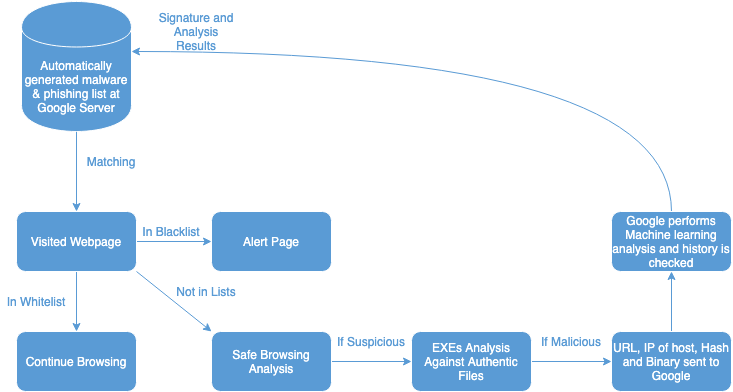
\includegraphics[width=0.95\textwidth]{google_safe_browsing.png}
	\caption{
		Architecture of Google Safe Browsing
		\citep{Priyam_Sandhu}}
	\label{fig:GSB_ARCHITECTURE}
\end{figure}

\begin{singlespace}
	\begin{table}[!b]
		\begin{center}
			\begin{tabular}{  m{11.9em}  m{11.9em}  m{11.9em}  } \toprule

				\multicolumn{1}{c}{\textbf{Version 1}}  &
				\multicolumn{1}{c}{\textbf{Version 2} } &
				\multicolumn{1}{c}{\textbf{Version 3}}                                                                                              \\ \midrule

				The hashing algorithm used in this
				version is MD5.                         & The hashing algorithm used in this
				version is SHA 256.                     & To improve the efficiency, protocol buffers are
				used by encoding the chunk data.\newline                                                                                            \\

				The efficiency is less and it is not
				scalable. \newline                      & In the place of a single versioned
				list, a series of "chunks” is used.     & Message Authentication Code (MAC) support
				is eliminated.                                                                                                                      \\

				The entire phishing list entries are to be
				downloaded at once because the
				partial list updates are not supported
				till the time the user fully downloads
				the recent version of list. \newline    & A list of URLs is received when the
				list of chunks is communicated
				while updating.                         & The API key format is modified. The Google
				Developers Console manages the API keys..                                                                                           \\

				The phishing data is given to the client in
				an order from old to new. For the
				phishing sites it is inefficient as they
				have a short lifetime.                  & The Chunks present are 32-bit
				truncated hashes                        & To differentiate between the kinds of sites and
				to allow more warnings, metadata
				functionality was used by Google-malware-
				shavar list.                                                                                                                        \\

				As regular updates are required, so the
				bandwidth consumption is escalated.     & As soon as a match is discovered,
				the 32 bit chunk is
				communicated to Google and in
				return a list of 256 bit hash is
				acquired.                               & For the full hash, modifications are carried out
				in the cashing semantics.                                                                                                           \\

				It is time consuming as the users scarcely
				find a match with the present pattern.  & As compared to version 1, it is
				faster                                  & An expiration time is included in the HTTP
				Response for Full-Length Hashes in
				response \newline                                                                                                                   \\

				It is slow and has high latency.        & It has improved speed and reduced
				Latency.                                & When an update request is sent, each time the
				clients are required to wash off cashed full
				length hashes \newline                                                                                                              \\

				                                        &                                                  & Optional metadata was included in HTTP
				Response for Full-Length Hashes  \newline                                                                                           \\

				                                        &                                                  & Host keys are not used.                \\\bottomrule
			\end{tabular}
			\caption{A comparison of Google Safe Browsing versions \citep{Priyam_Sandhu}}
			\label{tab:GSB_VERSIONS}
		\end{center}
	\end{table}
\end{singlespace}

\cite{Priyam_Sandhu} describes the mechanism behind GSB and captures the differences between the different API versions. However, the study dates back to 2015, and as a consequence, the version comparison table includes only the first three versions (Table \ref{tab:GSB_VERSIONS}). Since then, version four has been released, marking the end of support for version two and three.
\cite{Google} does not mention any fundamental changes to the version four API but details a series of adjustments focusing towards the growth in usage of mobile devices. The new API is optimised around the challenges of the mobile environment: the limited power, network bandwidth and poor quality of service. Moreover, the protection per bit is maximised, due to cellular data being a direct expense of the user.

Moving to performance assessment, \cite{Nikos_Virvilis} present a thorough evaluation of anti-phishing detection systems embedded in different browsers and on different platforms. In developing the proposed proof of concept security proxy, \cite{Nikos_Virvilis}

\begin{center}
	\small
	\begin{tabularx}{\textwidth}{  X  X  X  }\toprule
		                                 & \textbf{True positives} & \textbf{False negatives} \\ \midrule
		\textbf{IE (Windows)}            & 48.4\%                  & 9.9\%                    \\

		\textbf{Opera (Windows)}         & 77.9\%                  & 8.4\%                    \\

		\textbf{Chrome (Windows)}        & 93.0\%                  & 1.3\%                    \\

		\textbf{Firefox (Windows)}       & 86.7\%                  & 5.9\%                    \\

		\textbf{Opera mobile (Android)}  & 75.9\%                  & 7.9\%                    \\

		\textbf{Firefox mobile(Android)} & 85.4\%                  & 3.4\%                    \\

		\textbf{Safari mobile (iOS)}     & 38.7\%                  & 26.4\%                    \\\bottomrule
	\end{tabularx}
	\captionsetup{type=table}\caption{\label{tab:APDS_COMPARISON}Comparison of browser anti-phishing detection systems \citep{Nikos_Virvilis}}

\end{center}

{\parindent0pt uncovered the classification accuracy issues of popular browsers. The study compiles information on the substantial difference between phishing URL detection and malicious URL detection (Table \ref{tab:APDS_COMPARISON}). It is noticeable that from all the browsers that use GSB, Google Chrome is the better performer.}

\subsection{Motivation revision}
\label{subsec:motivation_revision}
The literature shows an exceptional level of creativity in the solutions it proposes. However, the work presented in this chapter focuses on raising the bar as high as possible regarding accuracy. Although this is a valuable target to aim for, none of them aims to improve upon existing browser protection in a manner that fits the context and prioritises of such system.


\section{Chapter overview}
This chapter outlined the status quo of the relevant literature, expanding on the essential takeaways of each study presented. As presented, the subject of phishing is not only prevalent in the field of security, but it reaches the psychology literature and more. The features and mechanisms considered as most effective by the studies presented in the rule-based and machine learning-based solutions will shape the design of the artefact.
